\chapter{Two-particle momentum probability distribution} \label{app:momDistDer}
\section{Standard form} \label{sec:standardDist}
The following is a derivation of two particle relative momentum probability distribution function when the single-particle kinetic energies are allowed to extend to infinity.
A quick note on notation conventions, $f_p$ and $f_E$ are used to refer to the momentum and energy forms of the distributions respectively.
Additionally, since we will be discussing the single-particle and two-particle distributions at length, each distribution is labeled by a subscript one or two so it is apparent what the physical system under consideration is.
Function with hat accents ($\,\hat{ }\,$) are used to denote that they are truncated forms of the equation.
As an example, the function describing the truncated relative collision energy distribution is labeled by $\hat{f}_\text{E,two}$.

Starting with the single-particle Maxwell-Boltzmann momentum probability distribution function for a gas of temperature $T$ with particles of mass $m$.
\begin{equation} 
\label{eq:single_particle_prob}
		 f_\text{p,one}( \vec{p} ) = \left(\frac{1}{2 \pi m k_B T}\right)^{3/2} \exp{ \frac{-p^2}{2 m k_B T} }
\end{equation}
This distribution is valid for any momentum $\vec{p}$ under the requirement that 
\begin{equation}
	\int_{-\infty}^\infty dp_x \,\int_{-\infty}^\infty dp_y \,\int_{-\infty}^\infty dp_z \, f_\text{p,one}( \vec{p} ) = 1
\end{equation}

Extension of this distribution into the two-particle regime may generally be complicated if a particle's trajectory is dependent on other particles trajectories (i.\,e.\;particles retain a "memory" of past collisions.) 
If, however, we assume that particle collisions are rapid and therefore largely independent of one another, we can approximate the two-particle momentum distribution as the product of two single particle functions \cite{Chliamovitch2017,Ehrenfest2015}. 
The two particle momentum distribution for a homogeneous system is then
\begin{equation}
\label{eq:two_particle_prob}
\begin{split}
		 f_\text{p,two}( \vec{p}_1, \vec{p}_2 ) &= f_\text{p,one}( \vec{p}_1 ) f_\text{p,one}( \vec{p}_2 ) \\
		  &= \left(\frac{1}{2 \pi m k_B T}\right)^3 \exp{\frac{-(p_1^2 + p_2^2)}{2 m k_B T}}
\end{split}
\end{equation}
Next, we'd like to consider a center-of-mass frame for the distribution. 
So we define
\begin{align*}
	\vec{p}_\text{C} & = \vec{p}_1 + \vec{p}_2             &	M   &= m_1 + m_2 = 2m \\
	\vec{p}_\text{R} & = \frac{\vec{p}_1 - \vec{p}_2}{2}   &   \mu &= \frac{m_1 m_2}{m_1 + m_2} = \frac{m}{2}
\end{align*}
From these equations we can use conservation of energy to determine the quadrature sum of the two momenta
\begin{align*}
	\frac{p_1^2}{2m} + \frac{p_2^2}{2m} &= \frac{p_\text{C}^2}{2M} + \frac{p_\text{R}^2}{2\mu} \\
	p_1^2 + p_2^2 &= \frac{p_\text{C}^2}{2} + 2 p_\text{R}^2
\end{align*}
Thus the two particle momentum probability distribution takes the form
\begin{equation} \label{eq:two_particle_prob_inf_atomFrame}
		 f_\text{p,two}( \vec{p}_\text{C}, \vec{p}_\text{R} ) = \left(\frac{1}{2 \pi M k_B T}\right)^{3/2} \left(\frac{1}{2 \pi \mu k_B T}\right)^{3/2} 
		 \exp{\frac{-p_\text{C}^2}{2 M k_B T}} \exp{\frac{-p_\text{R}^2}{2 \mu k_B T}}
\end{equation}
The relative collision energy distribution is found by integrating over the center-of-mass momentum.
\begin{equation}
\label{eq:relEnergy_inf}
\begin{split}
	\hat{f}_\text{p,two}(\vec{p}_{\text{R}}) &= \int d^3\vec{p}_\text{C} \, f_\text{p,two}(\vec{p}_\text{C},\vec{p}_\text{R}) \\
	&= \left( \frac{1}{2 \pi \mu k_B T} \right)^{3/2} \exp{\frac{-p_\text{R}^2}{2 \mu k_B T}}
\end{split}
\end{equation}


\section{Truncated form}\label{sec:truncDist}
Now let's consider the effects on the two-particle relative distribution when the single-particle Maxwell-Boltzmann distributions are truncated.
Starting from Eq.\,\ref{eq:two_particle_prob}, the two-particle momentum distribution may be written as
\begin{equation}
\begin{split}
	\hat{f}_\text{p,two} (\vec{p}_1, \vec{p}_2) &= \mathcal{N} \left(\frac{1}{2 \pi m k_B T}\right)^3 \exp{ \frac{-(p_1^2 + p_2^2)}{2 m k_B T}} \\ &\quad\quad \times \heaviside{\epsilon_\text{max} - \frac{p_1^2}{2m}} \heaviside{\epsilon_\text{max} - \frac{p_2^2}{2m}}
\end{split}
\end{equation}
We have modified the continuous distribution with a normalization constant $\mathcal{N}$ and Heaviside functions to enforce the truncation for each single particle kinetic energy.
The truncation energy, $\epsilon_\text{max}$, is here consider to be the same for both particles.
The normalization constant $\mathcal{N}$ is included to ensure that integration over the truncated probability distribution remains equal to one and will be found explicitly at the end of the derivation.
%The Heaviside function also 
%The meaning of $_r$ is such that f should be evaluated at each point in space. Furthermore since the atoms are held in a trapping potential, each point in space has a local trap depth relative to the lip at the top of the trap as shown in Fig.\,\ref{fig:haloTrapModel}

Once more, we are interested in the distribution of relative momenta so following our previous steps for the continuous distribution, we perform a change of variables to a center-of-mass frame so we can integrate out the center-of-mass component.
\begin{equation}
\begin{split}
	 \hat{f}_\text{p,two}(\vec{p}_{\text{R}}) & = \int d^3 \vec{p}_\text{C} \; \hat{f}_{\text{p,two}} (\vec{p}_1, \vec{p}_2) \\
	 &= \mathcal{N} \left(\frac{1}{2 \pi M k_B T}\right)^{3/2} \left(\frac{1}{2 \pi \mu k_B T}\right)^{3/2} \int d^3 \vec{p}_\text{C} \; \exp{\frac{-p_\text{C}^2}{2 M k_B T}} \exp{\frac{-p_\text{R}^2}{2 \mu k_B T}} \\ 
	 &\quad\quad \times \; 
	 \heaviside{\epsilon_\text{max} - \frac{p_\text{C}^2}{8m} - \frac{p_\text{R}^2}{2m} - \frac{\vec{p}_\text{C} \cdot \vec{p}_\text{R}}{2m}} 
	 \heaviside{\epsilon_\text{max} - \frac{p_\text{C}^2}{8m} - \frac{p_\text{R}^2}{2m} + \frac{\vec{p}_\text{C} \cdot \vec{p}_\text{R}}{2m}} 
\end{split}
\end{equation}
We expect isotropically distributed center-of-mass momenta so we integrate by transforming into spherical coordinates with the radius aligned along the interatomic axis
\begin{equation}
\begin{split}
	 \hat{f}_\text{p,two}(\vec{p}_{\text{R}}) &= \mathcal{N} \left(\frac{1}{2 \pi M k_B T}\right)^{3/2} \left(\frac{1}{2 \pi \mu k_B T}\right)^{3/2} \,\exp{\frac{-p_\text{R}^2}{2 \mu k_B T}} \\
	 &\quad\quad \times \; \int_0^{\pi} \sin \theta d\theta \int_0^{2\pi} d\phi \int_0^{\infty} dp_\text{C} \; p_\text{C}^2 \; \exp{\frac{-p_\text{C}^2}{2 M k_B T}} \\ 
	 &\quad\quad\quad \times \; \heaviside{\epsilon_\text{max} - \frac{p_\text{C}^2}{8m} - \frac{p_\text{R}^2}{2m} - \frac{p_\text{C} \, p_\text{R} \cos \theta}{2m}} \heaviside{\epsilon_\text{max} - \frac{p_\text{C}^2}{8m} - \frac{p_\text{R}^2}{2m} + \frac{p_\text{C} \, p_\text{R} \cos \theta}{2m}} 
\end{split}
\end{equation}
Making a change of variables
\begin{equation*}
\begin{split}
	X  &= \cos \theta \\
	dX &= - \sin \theta d \theta
\end{split}
\end{equation*}
Substitute and integrate over $\phi$
\begin{equation}
\begin{split}
	 \hat{f}_\text{p,two}(\vec{p}_{\text{R}}) &= 2 \pi \mathcal{N} \left(\frac{1}{2 \pi M k_B T}\right)^{3/2} \left(\frac{1}{2 \pi \mu k_B T}\right)^{3/2} \exp{\frac{-p_\text{R}^2}{2 \mu k_B T}} \\
	 &\quad\quad \times \; \int_{-1}^1 dX \int_0^{\infty} dp_\text{C} \; p_\text{C}^2 \; \exp{\frac{-p_\text{C}^2}{2 M k_B T}} \\ 
	 &\quad\quad\quad \times \; \heaviside{\epsilon_\text{max} - \frac{p_\text{C}^2}{8m} - \frac{p_\text{R}^2}{2m} - \frac{p_\text{C} \, p_\text{R} X}{2m}} \heaviside{\epsilon_\text{max} - \frac{p_\text{C}^2}{8m} - \frac{p_\text{R}^2}{2m} + \frac{p_\text{C} \, p_\text{R} X}{2m}} 
\end{split}
\end{equation}
Here we recognize that the two Heaviside functions cancel each other out on either side of the $dX$ integral.
However, since $\cos\theta$ is symmetric we may eliminate one of the Heaviside's, change the bounds of integration to go from $0 \rightarrow 1$, and multiply by two without changing the final result.
\begin{equation}
\begin{split}
	 \hat{f}_\text{p,two}(\vec{p}_{\text{R}}) &= 4 \pi \mathcal{N} \left(\frac{1}{2 \pi M k_B T}\right)^{3/2} \left(\frac{1}{2 \pi \mu k_B T}\right)^{3/2} \exp{\frac{-p_\text{R}^2}{2 \mu k_B T}} \\
	 &\quad\quad \times \; \int_{0}^1 dX \int_0^{\infty} dp_\text{C} \; p_\text{C}^2 \; \exp{\frac{-p_\text{C}^2}{2 M k_B T}} \; \heaviside{\epsilon_\text{max} - \frac{p_\text{C}^2}{8m} - \frac{p_\text{R}^2}{2m} - \frac{p_\text{C} \, p_\text{R} X}{2m}}
\end{split}
\end{equation}
At this point we can group the effects of truncation into a new function $\hat{\mathcal{G}}_\text{p}$ and rewrite using the continuous relative momentum probability distribution $f_\text{p,two}(\vec{p}_\text{R})$, Eq.\,\ref{eq:relEnergy_inf}.
\begin{equation}
\begin{split}
	 \hat{f}_\text{p,two}(\vec{p}_{\text{R}}) &= \left(\frac{1}{2 \pi \mu k_B T}\right)^{3/2} \exp{\frac{-p_\text{R}^2}{2 \mu k_B T}} \hat{\mathcal{G}}_\text{p}(\epsilon_\text{max}, \vec{p}_\text{R}) \\
	 &= f_\text{p,two}(\vec{p}_\text{R}) \, \hat{\mathcal{G}}_\text{p}(\epsilon_\text{max}, \vec{p}_\text{R})
\end{split}
\end{equation}
where $\hat{\mathcal{G}}_\text{p}(\epsilon_\text{max}, \vec{p}_\text{R})$ is given by
\begin{equation} \label{eq:mom_dist_st_3}
\begin{split}
	\hat{\mathcal{G}}_\text{p}(\epsilon_\text{max}, \vec{p}_\text{R}) &= 4 \pi \mathcal{N} \left(\frac{1}{2 \pi M k_B T}\right)^{3/2} \int_{0}^1 dX \int_0^{\infty} dp_\text{C} \; p_\text{C}^2 \; \exp{\frac{-p_\text{C}^2}{2 M k_B T}} \\
	 &\quad\quad \times \; \heaviside{\epsilon_\text{max} - \frac{p_\text{C}^2}{8m} - \frac{p_\text{R}^2}{2m} - \frac{p_\text{C} \, p_\text{R} X}{2m}}
\end{split}
\end{equation}

In photoassociation we are interested in the relative collision energy distribution $f_\text{E,two}(\epsilon)$.
Assuming the distribution of momenta are isotropic, we change variables once more using
\begin{align*}
	\epsilon &= \frac{p_\text{R}^2}{2 \mu} &\quad \mathcal{E}  &= \frac{p_\text{C}^2}{2 M} \\
	p_\text{R} &= \sqrt{2 \mu \epsilon}    &\quad p_\text{C} &= \sqrt{2 M \mathcal{E}} \\
	dp_\text{R} \, p_\text{R}^2 &= \sqrt{2 \mu^3 \epsilon} \, d\epsilon 	&\quad	dp_\text{C} \, p_\text{C}^2 &= \sqrt{2 M^3 \mathcal{E}} \, d \mathcal{E}
\end{align*}
Using these expressions and noting that 
\begin{equation}
\begin{split}
	\int d^3\vec{p}_\text{R} \, f_\text{p,two}(\vec{p}_\text{R}) = \int d \epsilon \, f_\text{E,two}(\epsilon) = 1 \\
	\Rightarrow 4 \pi \, p_\text{R}^2 \, f_\text{p,two}(\vec{p}_\text{R}) \, dp_\text{R} = f_\text{E,two}(\epsilon) \, d \epsilon
\end{split}
\end{equation}
Then $\hat{f}_\text{E,two}(\tilde{\epsilon})$ is given by
\begin{equation} \label{eq:mom_dist_st_4}
\begin{split}
	\hat{f}_\text{E,two}(\epsilon) = \mathcal{N} \frac{2}{\sqrt{\pi}} \, \frac{\sqrt{\epsilon}}{(k_B T)^{3/2}} \, e^{-\epsilon/k_B T} \int_0^1 dX \int_0^\infty d \mathcal{E} \, \frac{2}{\sqrt{\pi}} \, \frac{\sqrt{\mathcal{E}}}{(k_B T)^{3/2}} \, e^{-\mathcal{E} / k_B T} \\
	\times \heaviside{\epsilon_\text{max} - \frac{\mathcal{E} - \epsilon}{2} - X \sqrt{\mathcal{E} \,  \epsilon}}
\end{split}
\end{equation}
We can now determine the normalization constant $\mathcal{N}$ by requiring that
\begin{equation*}
	\int_0^{2 \, \epsilon_\text{max}} d \epsilon \, \hat{f}_\text{E,two}(\epsilon) = 1
\end{equation*}
where we have used an energy cutoff of $2 \, \epsilon_\text{max}$ since either particle may have an energy in the range $[0 \rightarrow \epsilon_\text{max}]$. 
With the normalization, the complete expression for $\hat{f}_\text{E,two}(\epsilon)$ is then
\begin{equation} \label{eq:truncRelDist}
	\hat{f}_\text{E,two}(\epsilon) = \frac{2}{\sqrt{\pi}} \, \frac{\sqrt{\epsilon}}{(k_B T)^{3/2}} \, \exp{\frac{-\epsilon}{k_B T}} \, \hat{\mathcal{G}}_E(\epsilon_\text{max}, \epsilon)
\end{equation}
where all the effects of the truncation have been moved to $\hat{\mathcal{G}}_E$, given by 
\begin{equation} \label{eq:truncWeighting}
\hspace*{-3cm} 
	\hat{\mathcal{G}}_E(\epsilon_\text{max}, \epsilon) = \frac{\displaystyle
	\int_0^\infty d \mathcal{E} \, \frac{2}{\sqrt{\pi}} \, \frac{\sqrt{\mathcal{E}}}{(k_B T)^{3/2}} \, e^{-\mathcal{E} / k_B T} \heaviside{\epsilon_\text{max} - \frac{\mathcal{E} - \epsilon}{2} - X \sqrt{\mathcal{E} \,  \epsilon}}}
	{\displaystyle \int_0^{2\,\epsilon_\text{max}} d \epsilon \frac{2}{\sqrt{\pi}} \, \frac{\sqrt{\epsilon}}{(k_B T)^{3/2}} \, e^{-\epsilon/k_B T} \int_0^1 dX \int_0^\infty d \mathcal{E} \, \frac{2}{\sqrt{\pi}} \, \frac{\sqrt{\mathcal{E}}}{(k_B T)^{3/2}} \, e^{-\mathcal{E} / k_B T} \heaviside{\epsilon_\text{max} - \frac{\mathcal{E} - \epsilon}{2} - X \sqrt{\mathcal{E} \,  \epsilon}}}
\end{equation}
As a check of the limiting behavior of $\hat{\mathcal{G}}_E$, we expect that $ \displaystyle \lim_{\epsilon_\text{max} \rightarrow \infty} \hat{\mathcal{G}}_E = 1$.
This is simply a requirement that for single-particle distributions where the truncation is large, then the truncated distribution should approach the untruncated distribution. 
This is trivial to verify, recalling that 
\begin{equation}
	\int_0^{\infty} dx \sqrt{x} e^{-x/x_0} = \frac{\sqrt{\pi}}{2} (x_0)^{3/2}
\end{equation}

Although the form of Eq.\,\ref{eq:truncWeighting} is rather cumbersome, this equation may be solved numerically.
Below are plots exploring the behavior of $\hat{f}_\text{E,two}(\epsilon)$ and $\hat{\mathcal{G}}_E$ as $\epsilon_\text{max}$ and $\epsilon$ are varied.
\begin{figure}
	\centerline{
	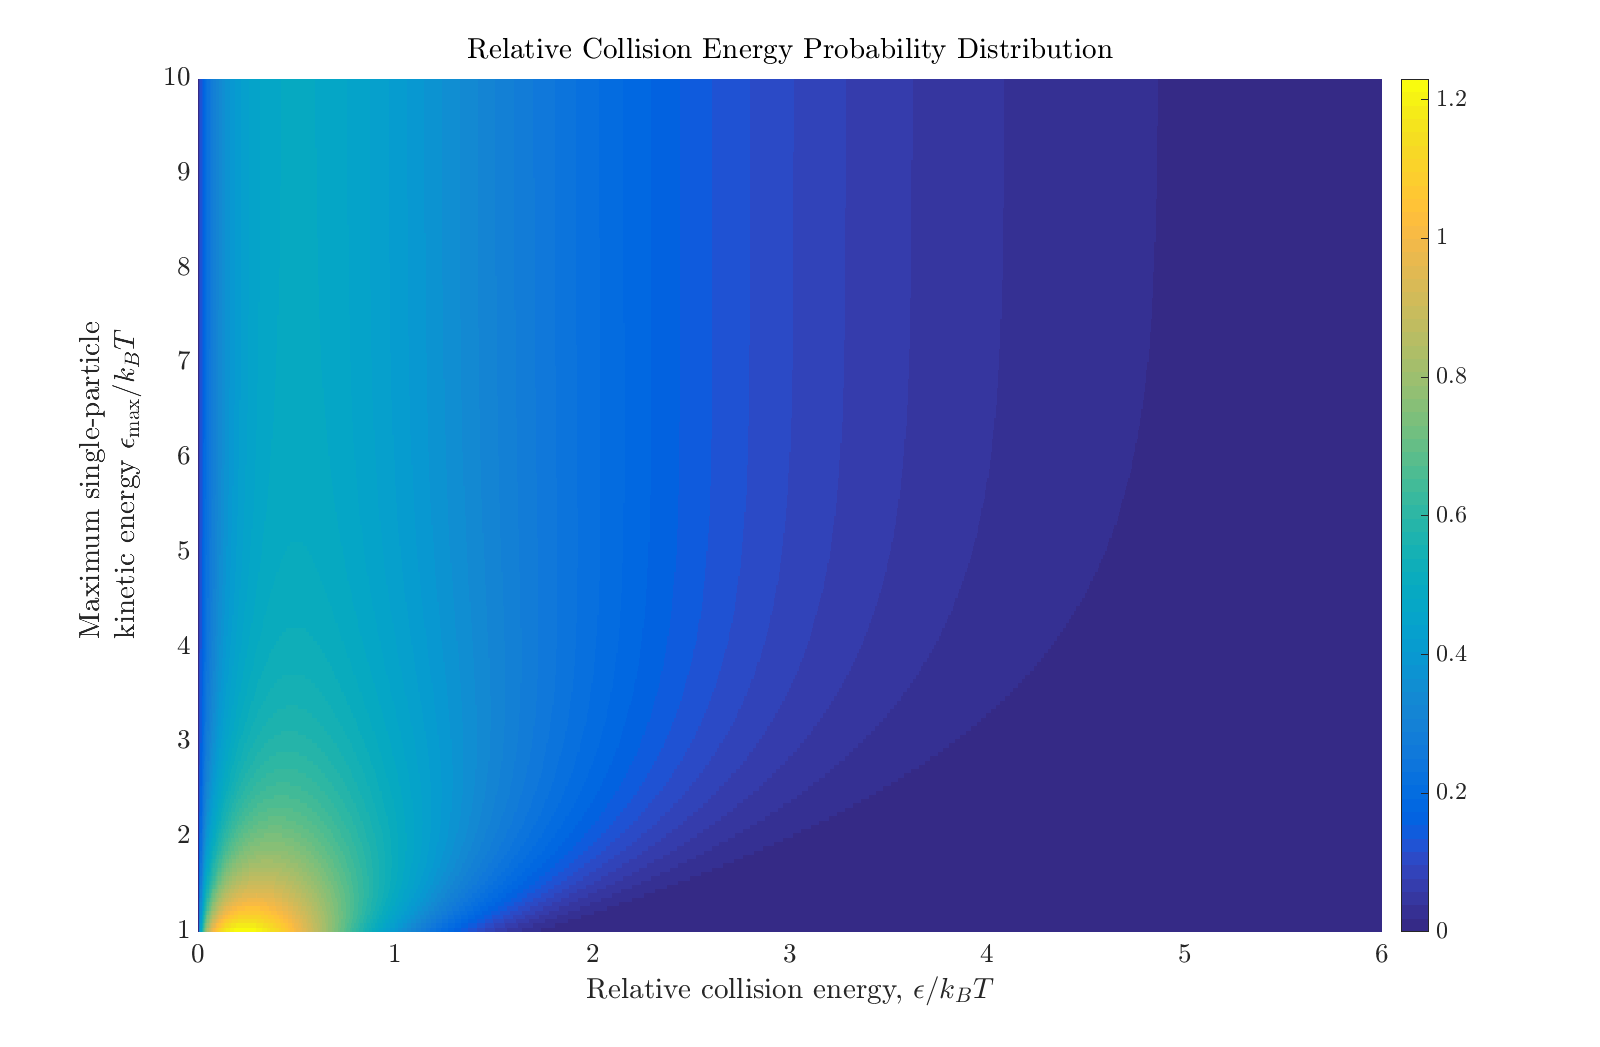
\includegraphics[width=\textwidth]{relativeColDistribution.png}}
	\caption{2D Surface plot of the relative collision likelihood}{$\hat{f}_\text{E,two}(\epsilon)$ is shown with energies scaled by the characteristic energy $k_B T$. The collision likelihood is given for relative collision energy along the bottom axis and the maximum single-particle kinetic energy $\epsilon_\text{max}$ increasing on the vertical axis. As required, there are no occupied energy states above $2\,\epsilon_\text{max}$ and once the maximum energy is greater than $\sim\!4$ the distribution behaves as expected and appears to become constant. This is discussed in Sec.\,\ref{sec:trunc_trap}.}
	\label{fig:momSurfRelCol}
\end{figure} 

\begin{figure}
	\centerline{
	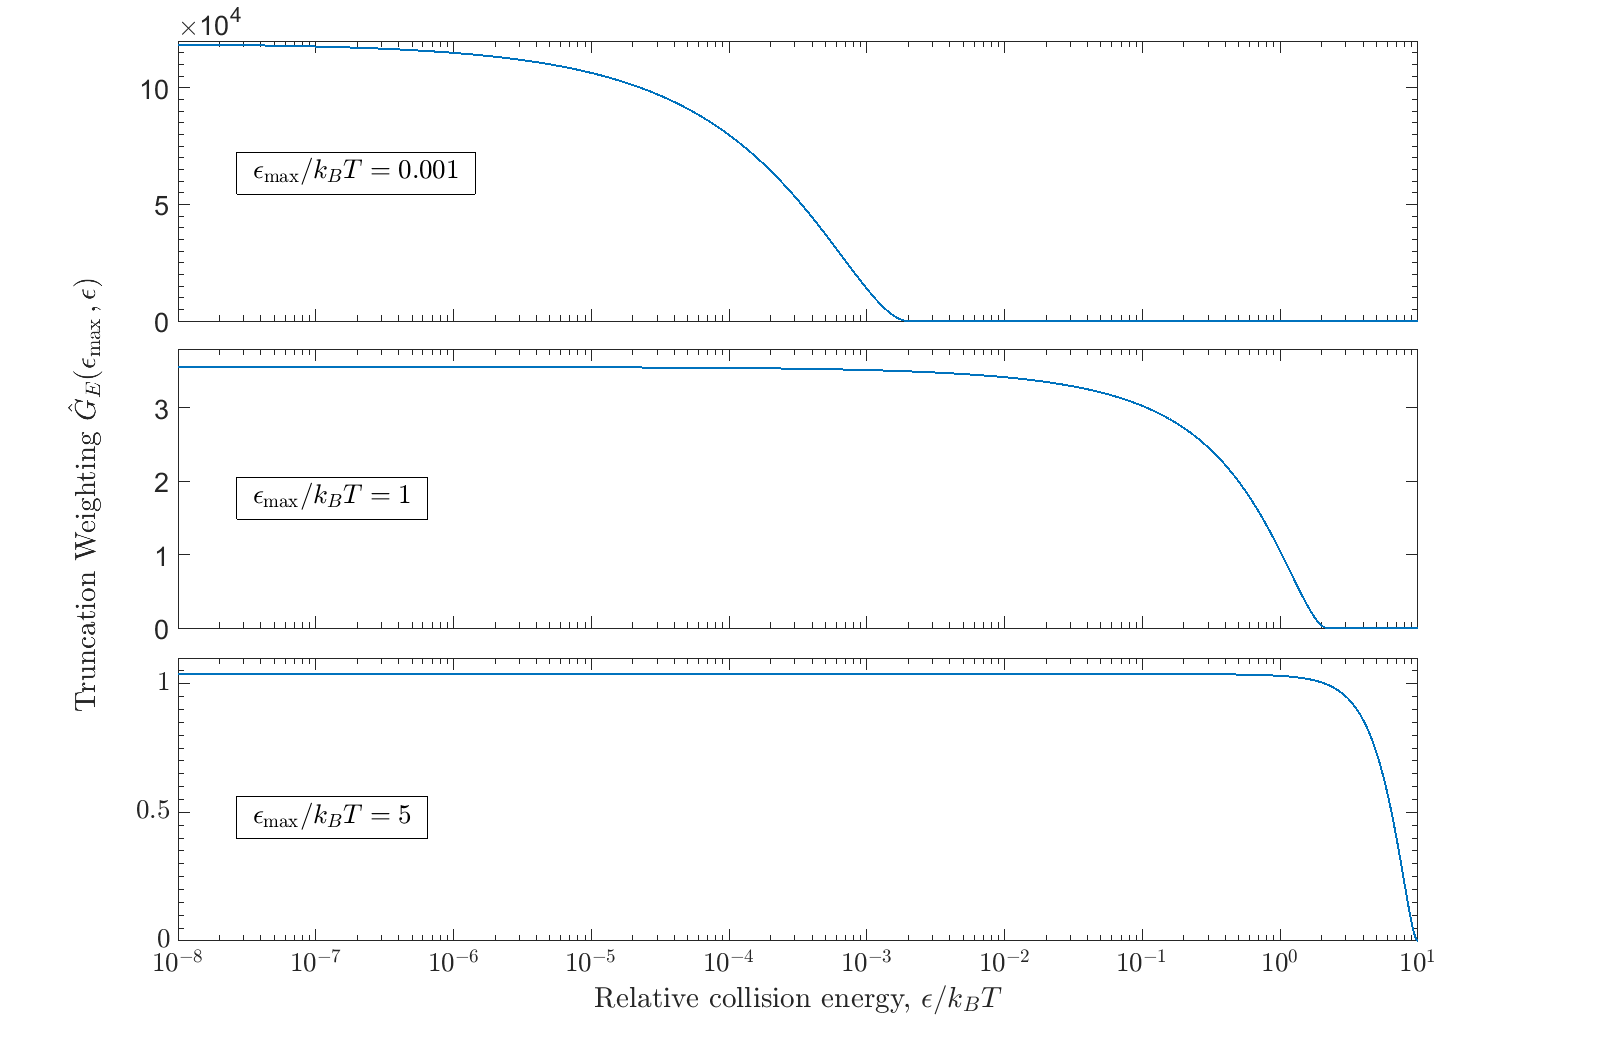
\includegraphics[height=0.4\textheight]{cutAcrossColE.png}}
	\caption{Behavior of $\hat{\mathcal{G}}_E(\epsilon_\text{max}, \epsilon)$ vs. collision energy}
	\label{fig:relColvsColE}
\end{figure} 

\begin{figure}
	\centerline{
	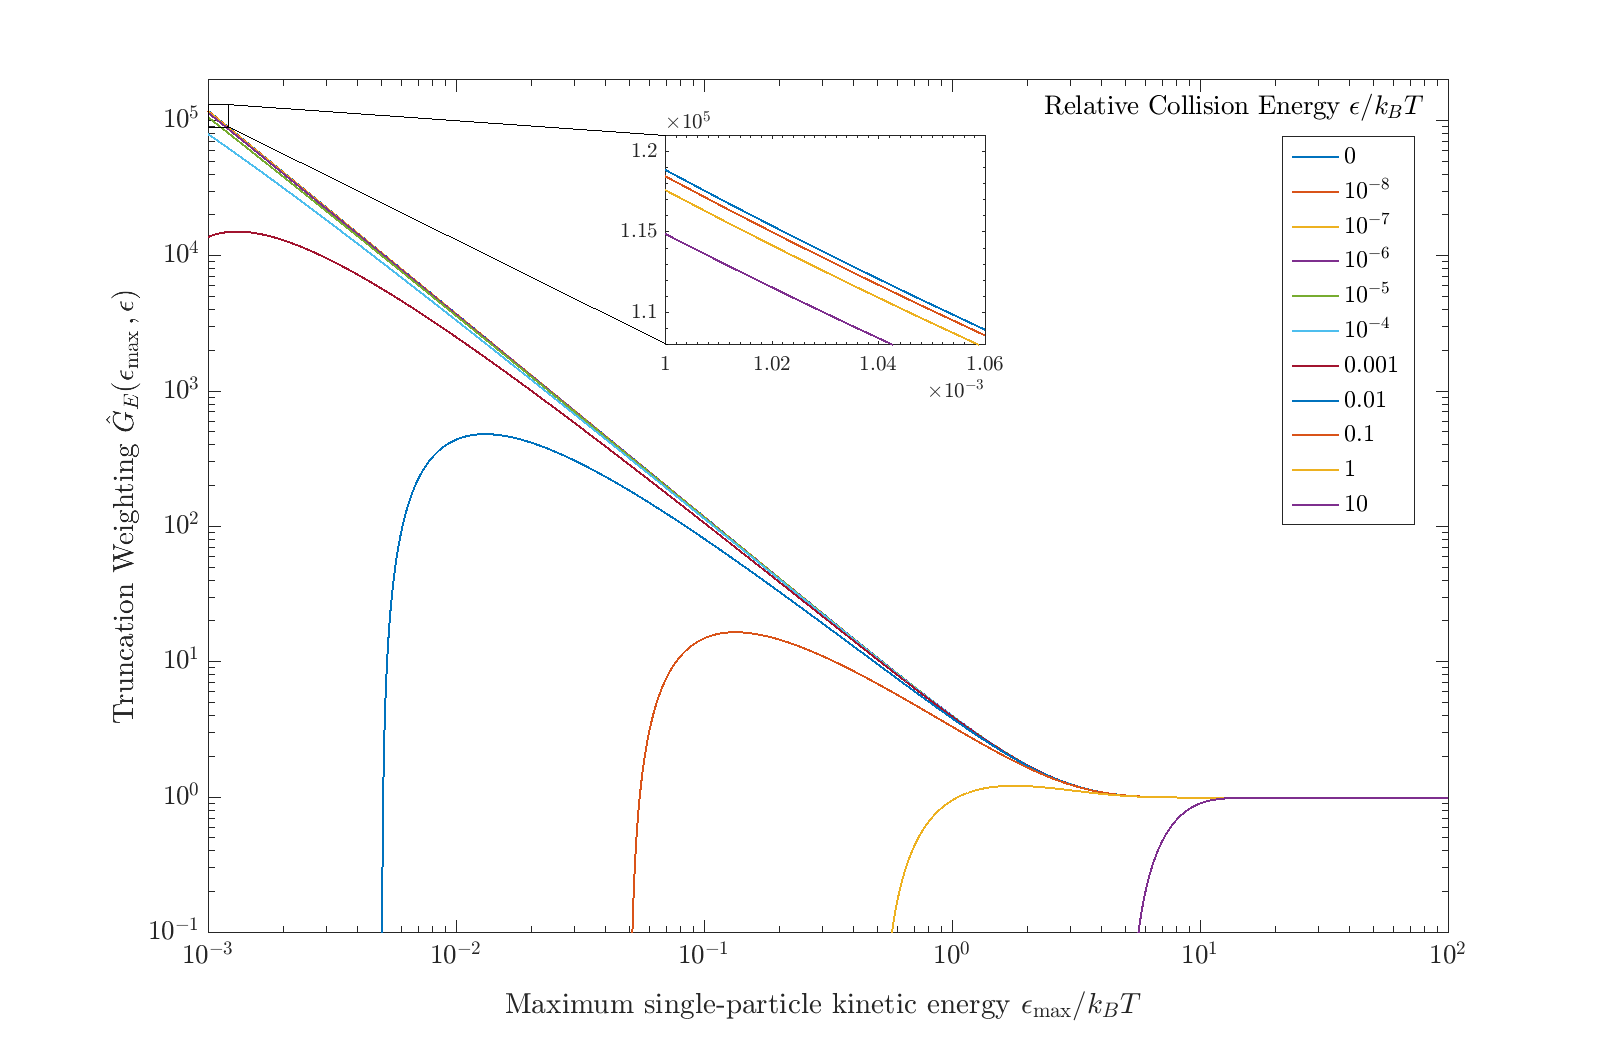
\includegraphics[height=0.4\textheight]{cutAcrossEta.png}}
	\caption{Behavior of $\hat{\mathcal{G}}_E(\epsilon_\text{max}, \epsilon)$ vs. $\epsilon_\text{max}$}
	\label{fig:relColvsEta}
\end{figure} 



%Plugging these expressions into Eq.\,\ref{eq:mom_dist_st_3} and rearranging
%\begin{multline}
%	\hat{f}_\text{E,two}(\tilde{\epsilon}) = \frac{2 \mathcal{N}}{\sqrt{\pi}} \frac{e^{-\tilde{\epsilon}}}{(2 \pi \mu k_B T)^{3/2}} \int_0^1 dX  \int_0^\infty d \tilde{E} \, e^{-\tilde{E}} \, \sqrt{\tilde{E}} \\
%	\times \heaviside{\epsilon_\text{max} - \frac{\tilde{E} - \tilde{\epsilon}}{2} - X \sqrt{\tilde{E} \,  \tilde{\epsilon}}}
%\end{multline}
%
%
%using $dp p^2$ given above we then write 
%\begin{equation} \label{eq:truncWeighting}
%\hspace*{-1cm} 
%	\hat{\mathcal{G}}_E(\epsilon_\text{max}, \epsilon) = \frac{\displaystyle
%	\int_0^1 dX \frac{2}{\sqrt{\pi}} \int_0^\infty d \tilde{E} e^{-\tilde{E}}\sqrt{\tilde{E}} \; \heaviside{\eta(\vec{r}) - \frac{\tilde{E}}{2} - \frac{\tilde{\epsilon}}{2} - X \sqrt{\tilde{E}\tilde{\epsilon}}}}
%	{\displaystyle \int_0^{2\eta(\vec{r})} d \tilde{\epsilon} \frac{2}{\sqrt{\pi}} \sqrt{\tilde{\epsilon}} \, e^{-\tilde{\epsilon}} \int_0^1 dX \frac{2}{\sqrt{\pi}} \int_0^\infty d \tilde{E} e^{-\tilde{E}}\sqrt{\tilde{E}} \; \heaviside{\eta(\vec{r}) - \frac{\tilde{E}}{2} - \frac{\tilde{\epsilon}}{2} - X \sqrt{\tilde{E}\tilde{\epsilon}}}}
%\end{equation}